\section{Assignment}
\subsection{Explain the physical meaning of $H_d$. How would you realize such a term?}
% Come vedete, per questa sezione non ho creato un nuovo file Sezione_3.tex, ma l'ho direttamente definita qua sotto. A seconda di come più vi aggrada, potete fare un file per ogni sezione e richiamarlo nel file principale con \input{}, oppure mettere tutto nello stesso file. It's up to you.

The physical meaning of $H_d$ is that of a coherent driving field that pumps the cavity mode at frequency $\omega$. This term represents the interaction between the cavity field and an external classical field, which can be realized experimentally by shining a laser beam into the cavity. The laser frequency $\omega$ is typically chosen to be close to the cavity resonance frequency $\omega_c$ to efficiently drive the cavity mode. The amplitude $\mathcal{E}$ characterizes the strength of the driving field, which can be controlled by adjusting the intensity of the laser.
\subsection{Rewrite the hamiltonian in the frame of the drive and use the RWA.}




We assume:
\begin{itemize}
    \item a small atomic decay rate into modes outside the cavity, denoted by $\Gamma$,
    \item a non-perfect cavity with photon loss rate $\kappa$.
\end{itemize}

\paragraph{A. Initial Hamiltonian ($\hat{H}$)}


The system Hamiltonian in the laboratory frame consists of the cavity field, a two-level atom, the atom–cavity interaction, and an external driving field:
\begin{equation}
\hat{H}
=
\hbar \omega_c a^\dagger a
+
\hbar \omega_a \ket{e}\bra{e}
+
\hbar \tilde{g} \left( \sigma^+ a + \sigma^- a^\dagger \right)
+
\varepsilon e^{i\omega t} a
+
\varepsilon^* e^{-i\omega t} a^\dagger .
\end{equation}

\noindent
\textbf{Parameters:}
\begin{itemize}
    \item $\omega = \omega_c = \omega_a$ (resonant driving),
    \item $\delta \approx 0$ and $\omega \gg \delta$.
\end{itemize}

\paragraph{B. Unitary Transformation ($R$)}

To move to the rotating frame, we define the unitary operator
\begin{equation}
R
=
e^{i \omega \ket{e}\bra{e} t}
\otimes
e^{i \omega a^\dagger a t}
\equiv
R_A \otimes R_{\mathrm{EM}} .
\end{equation}

The transformed Hamiltonian is given by
\begin{equation}
H'
=
R H R^\dagger
-
i \hbar R \dot{R}^\dagger .
\end{equation}

\paragraph{C. Expansion of the Transformation}

\subparagraph{I. Inertial Term}

Using
\begin{align}
R_A \dot{R}_A^\dagger &= - i \omega \ket{e}\bra{e}, \\
R_{\mathrm{EM}} \dot{R}_{\mathrm{EM}}^\dagger &= - i \omega a^\dagger a ,
\end{align}
we obtain
\begin{equation}
- i \hbar R \dot{R}^\dagger
=
- \hbar \omega a^\dagger a
-
\hbar \omega \ket{e}\bra{e}.
\end{equation}

\subparagraph{II. Transformation of the Hamiltonian Terms}

The field and atomic operators transform as
\begin{align}
a_H(t) &= R_{\mathrm{EM}} a R_{\mathrm{EM}}^\dagger = a e^{-i\omega t}, \\
\sigma_H(t) &= R_A \sigma R_A^\dagger = \sigma e^{-i\omega t}.
\end{align}

Applying $R H R^\dagger$ term by term:

\paragraph{Cavity Energy}
\begin{equation}
\mathbb{1} \otimes
R_{\mathrm{EM}} \, \hbar \omega_c a^\dagger a \, R_{\mathrm{EM}}^\dagger
=
\hbar \omega_c a^\dagger a .
\end{equation}

\paragraph{Atomic Energy}
\begin{equation}
R_A \, \hbar \omega_a \ket{e}\bra{e} \, R_A^\dagger \otimes \mathbb{1}
=
\hbar \omega_a \ket{e}\bra{e}.
\end{equation}

\paragraph{Interaction Terms}
\begin{align}
R_A \sigma^+ R_A^\dagger \otimes R_{\mathrm{EM}} a R_{\mathrm{EM}}^\dagger
&=
\sigma^+ e^{i\omega t} \otimes a e^{-i\omega t}
=
\sigma^+ a , \\
R_A \sigma^- R_A^\dagger \otimes R_{\mathrm{EM}} a^\dagger R_{\mathrm{EM}}^\dagger
&=
\sigma^- e^{-i\omega t} \otimes a^\dagger e^{i\omega t}
=
\sigma^- a^\dagger .
\end{align}

\paragraph{Driving Terms}
\begin{align}
\varepsilon e^{i\omega t} a_H(t) &= \varepsilon a , \\
\varepsilon^* e^{-i\omega t} a_H^\dagger(t) &= \varepsilon^* a^\dagger .
\end{align}

\paragraph{D. Final Hamiltonian in the Rotating Frame}

Defining the detunings
\[
\delta_c = \omega_c - \omega,
\qquad
\delta_a = \omega_a - \omega,
\]
the transformed Hamiltonian becomes
\begin{equation}\label{eq:rwaham}
H'
=
\hbar \delta_c a^\dagger a
+
\hbar \delta_a \ket{e}\bra{e}
+
\hbar g \left( \sigma^+ a + \sigma^- a^\dagger \right)
+
\mathcal{E} a
+
\mathcal{E}^* a^\dagger .
\end{equation}

\paragraph{Laboratory Frame Expression}

For reference, the Hamiltonian in the laboratory frame can be written as
\begin{equation}
H
=
\hbar \omega_c a^\dagger a
+
\hbar \omega_a \ket{e}\bra{e}
+
\hbar g \left( \sigma^+ a + \sigma^- a^\dagger \right)
+
\mathcal{E} a
+
\mathcal{E}^* a^\dagger .
\end{equation}

Consider the resonant case where
\[
\omega = \omega_a = \omega_c
\]
and assume no coupling between the cavity and the atom,
\[
\tilde{g} = 0.
\]
Given an initially empty cavity,
\[
\ket{g,0},
\]
we numerically solve the corresponding master equation at resonance (e.g.\ using the \texttt{QuTiP} library).

\subsection{Integrate the master equation for enough large times to find the steady state. What is the mean photon number $\langle \hat{a}^\dagger \hat{a} \rangle$? What is the steady-state occupation of the $n$-photon states? Plot the histogram of occupations and compare with a coherent state distribution. [Suggestion: work in a regime of parameters that allow you to keep the photon Hilbert space sufficiently small (e.g. max $10 - 50$ photon states) and the average photon number of the steady state small, $\langle \hat{a}^\dagger \hat{a} \rangle \le 10$. Explain how you made your choice.]}
Given the conditions of the last point,
\begin{itemize}
    \item $g=0$
    \item $w=w_c=w_a$
\end{itemize}
we can write the Hamiltonian \ref{eq:rwaham} as the following (using $\hbar=1$):
\begin{equation}
    H'= \mathcal{E} a
+
\mathcal{E}^* a^\dagger
\end{equation}
As we can see this Hamiltonian is time independent and it represent the continuous creation and destruction of photons caused by the pumping field.
We now can visualize the evolution of the expected values of the number of photons:
\begin{figure}[H]
    \centering
    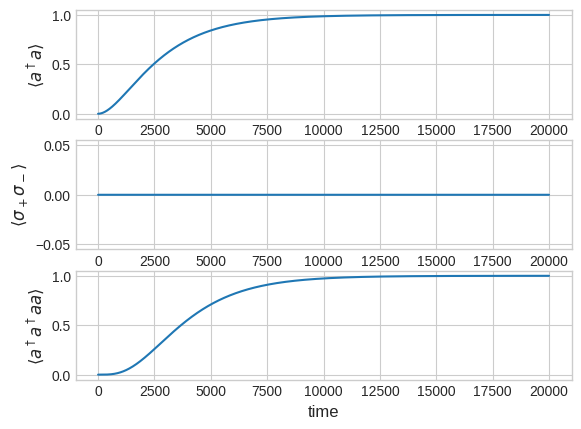
\includegraphics[width=0.5\linewidth]{Figure/expected_no_g.png}
    \caption{Time evolution of the expected values of the J-C model coupled with a bath}
    \label{fig:placeholder}
\end{figure}
Here we can see that the expected value of finding the atom in the excited state stays at 0 since there are no terms in the Hamiltonian that interact with the atom whereas the number of photons oscillates reaching an equilibrium by the final time. 
We also can visualize the different density matrices of the system along with occupation probabilities of each state when the system reach an equilibrium.
\begin{figure}[H]
    \centering
    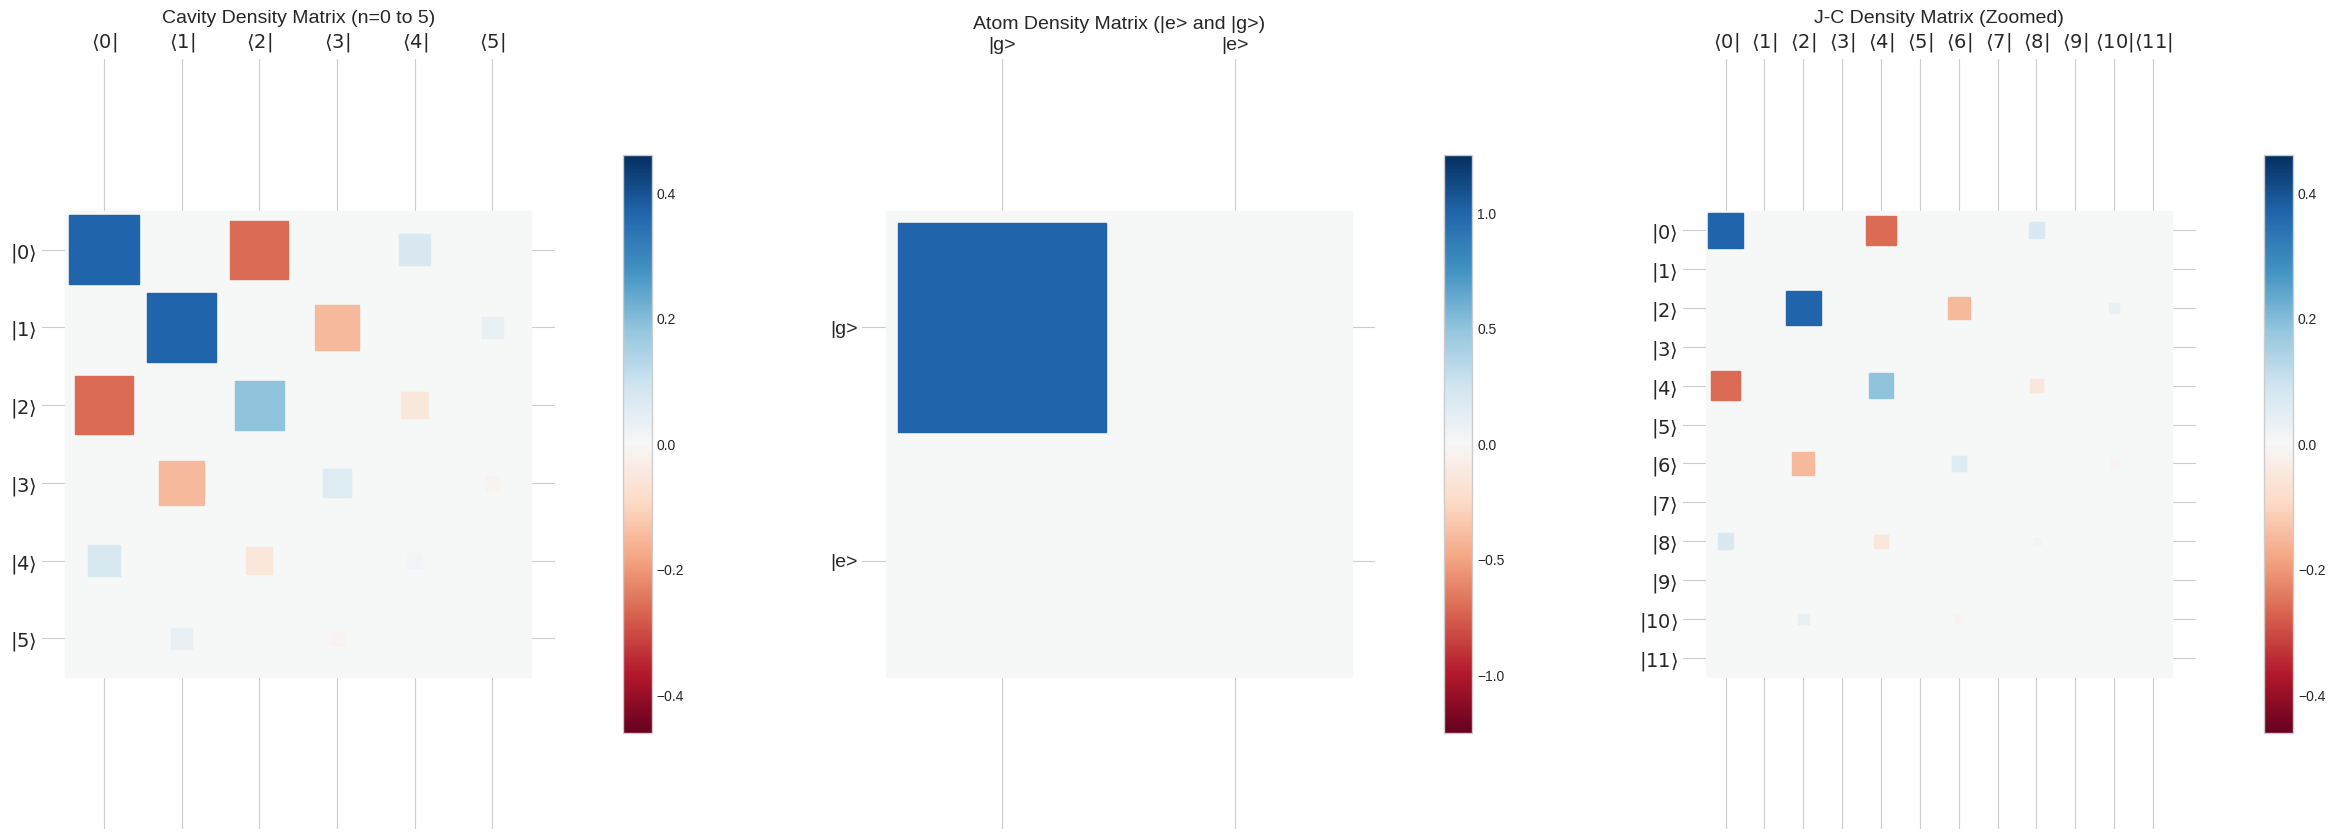
\includegraphics[width=0.75\linewidth]{Figure/dens_no_g.png}
    \caption{Different density matrices of the system}
    \label{fig:placeholder}
\end{figure}
It is noticeable that in this system the states where the atom can be in the excited states are empty (right plot). In order to compare this distribution with a coherent state distribution we can visualize the density matrix of a coherent state with the same average photon number as the one of the J-C model coupled with a bath:

\begin{figure}[H]
    \centering    
    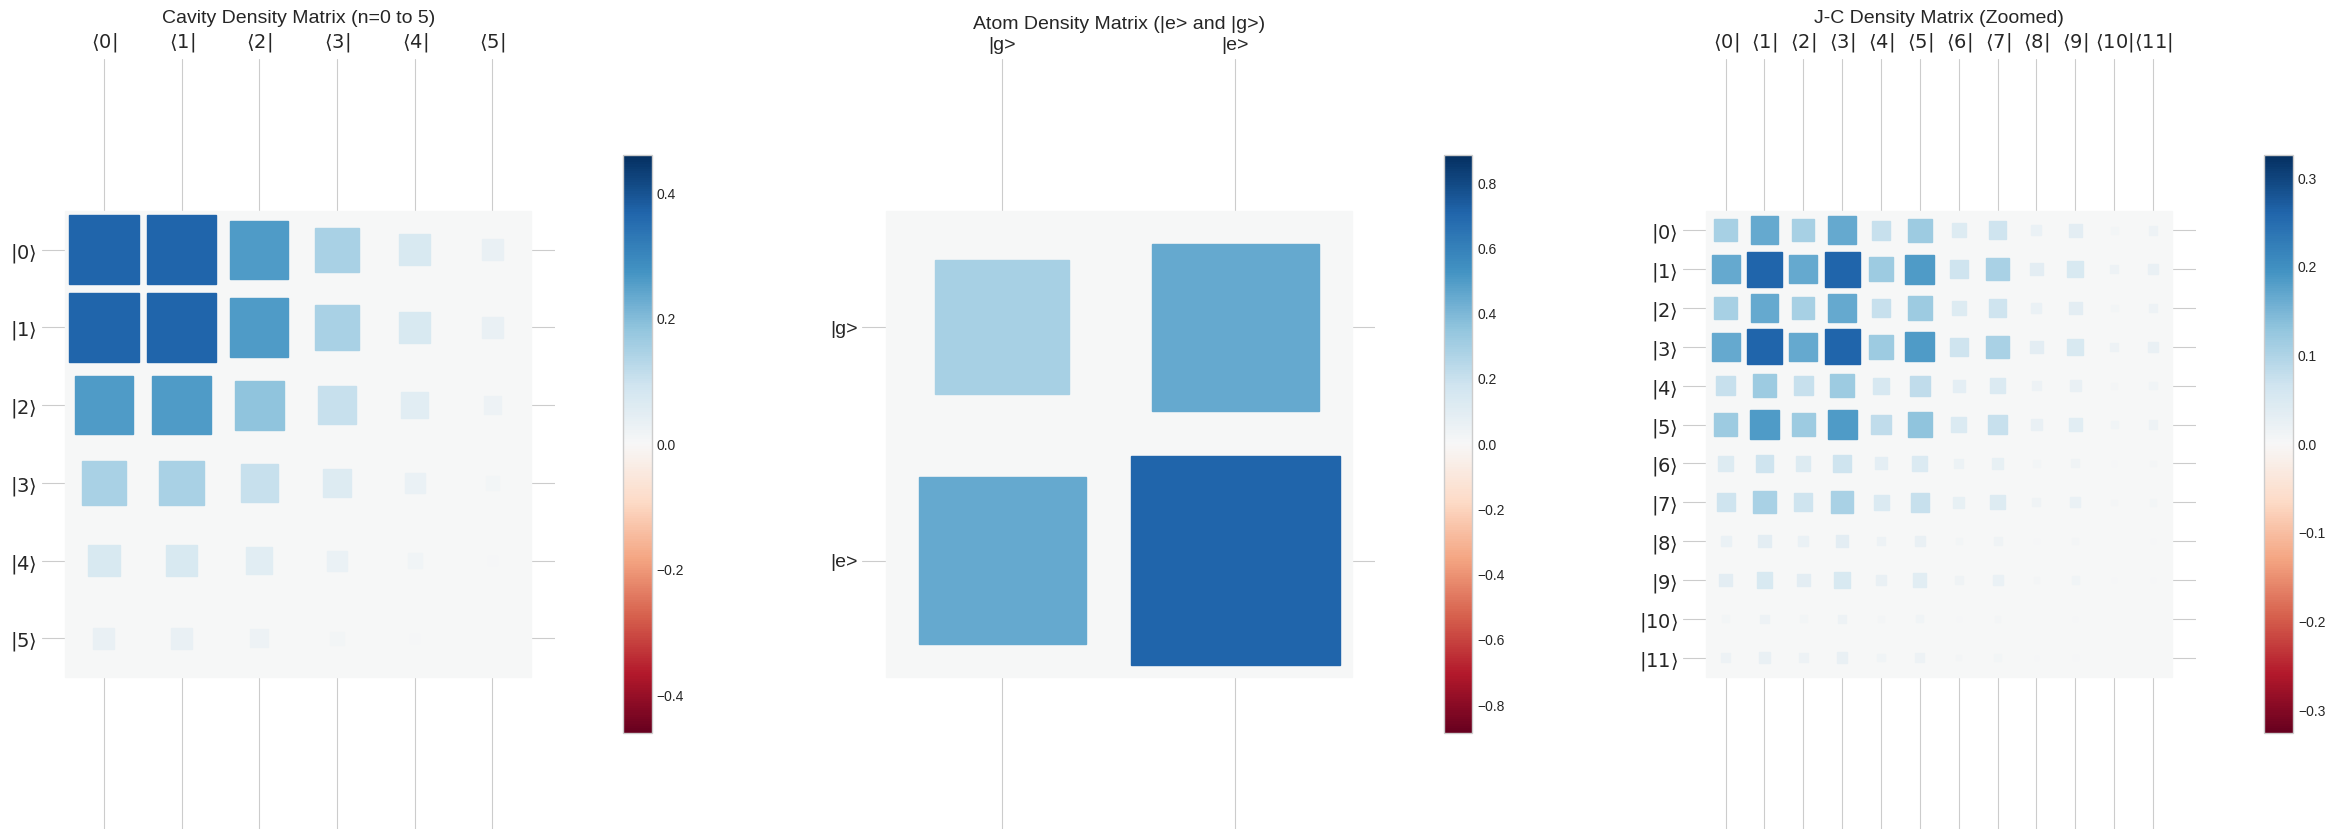
\includegraphics[width=0.75\linewidth]{Figure/dens_coh.png}
    \caption{Different density matrices of a coherent state}
    \label{fig:placeholder}
\end{figure}
The coherent state is defined as:
$$|\alpha\rangle = e^{-\frac{|\alpha|^2}{2}}\sum_{n=0}^\infty \frac{\alpha^n}{\sqrt{n!}} |n\rangle$$
Where $\alpha$ is a complex number that characterizes the state and $|n\rangle$ are the Fock states. The average photon number of a coherent state is given by $\langle \hat{a}^\dagger \hat{a} \rangle = |\alpha|^2$. In our case, we choose $\alpha$ such that the average photon number of the coherent state is the same as that of the J-C model coupled with a bath, in order to compare the two distributions.

If $\langle n \rangle \gg 1$ we get a normal distribution centered at $|\alpha|^2$, so we set $|\alpha|=1$, $\kappa=0.001$ getting a value of $\mathcal{E}=0.0005$ to maintain a low number of photons and a weak drive.

The density matrix of the coherent state is not diagonal in the Fock basis and the occupation probabilities of the different states follow a Poisson distribution. In order to compare the two distributions we can visualize the histogram of occupations for both cases:
\begin{figure}[H]
    \centering
    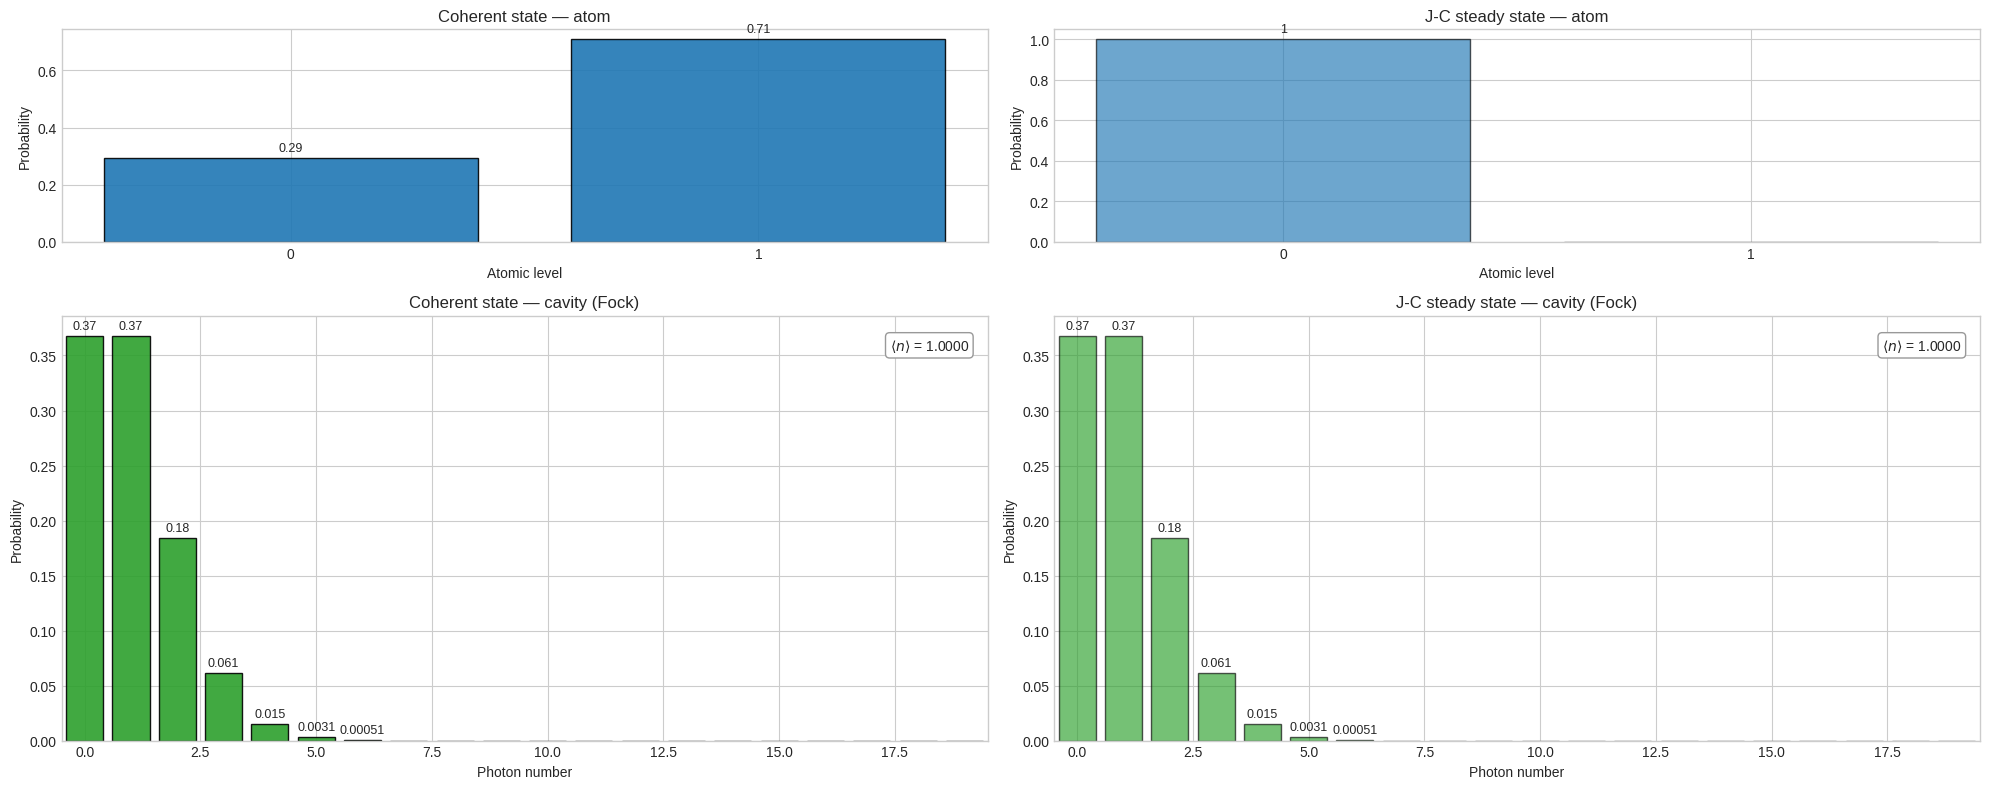
\includegraphics[width=0.75\linewidth]{Figure/hist_no_g.png}
    \caption{Comparison of the occupation probability of the different states with a coherent state}
    \label{fig:placeholder}
\end{figure}
As we can see the distribution of the occupation probabilities of the different states in the case of the J-C model coupled with a bath is very similar to the one of a coherent state. The choice of the parameters was made in order to keep the average photon number small $\approx 1$ and therefore to be able to visualize the occupation probabilities of the different states without having to consider a large number of photon states.

In this case the intensity of the drive $\mathcal{E}$ was chosen to be small since we want to study the weak drive regime, if the drive is too strong we get a perfect uniform distribution of the occupation probabilities of the different states, which is due to the impossibility of occupying more states (the maximum number of photons is set to  20) . Therefore we choose a value of $\mathcal{E}$ that allows us to have a non-trivial distribution of the occupation probabilities of the different states while keeping the average photon number small.

\subsection{In the presence of a coupling $\tilde{g}$, the previous resonance condition is not valid anymore. Set $\omega$ to resonance with the lowest (one-photon) dressed state of the Jaynes-Cummings model and find again the steady state in the strong-coupling condition $\tilde{g} \gg \Gamma, \kappa$ and weak drive $\mathcal{E}$. How important is the value of the pumping strength $\mathcal{E}$? (Be careful that increasing $\mathcal{E}$ too much could lead to instability/bistability)}

When the coupling $\tilde{g}$ is introduced, the degeneracy of the $n$-photon states is lifted, forming the \textbf{Jaynes-Cummings ladder}. To probe the blockade, we tune the drive frequency $\omega$ to the first rungs of the ladder, specifically $\omega = \omega_c \pm g$. In the strong-coupling condition ($g=100, \kappa=1, \Gamma=1$), the system enters the quantum regime.



As shown in the evolution plots, the steady-state mean photon number $\langle n \rangle$ is significantly lower than in the $g=0$ case. The value of the pumping strength $\mathcal{E}$ is critical:
\begin{itemize}
    \item If $\mathcal{E} \ll \kappa$, we stay in the single-photon regime, maximizing the blockade effect and we will see something that is closer to a coherent state.
    \item As $\mathcal{E}$ increases (up to $\mathcal{E}=0.5$), we observe a slight increase in $\langle n \rangle$, but it remains $\ll 1$.
\end{itemize}


\begin{figure}[H]
    \centering
    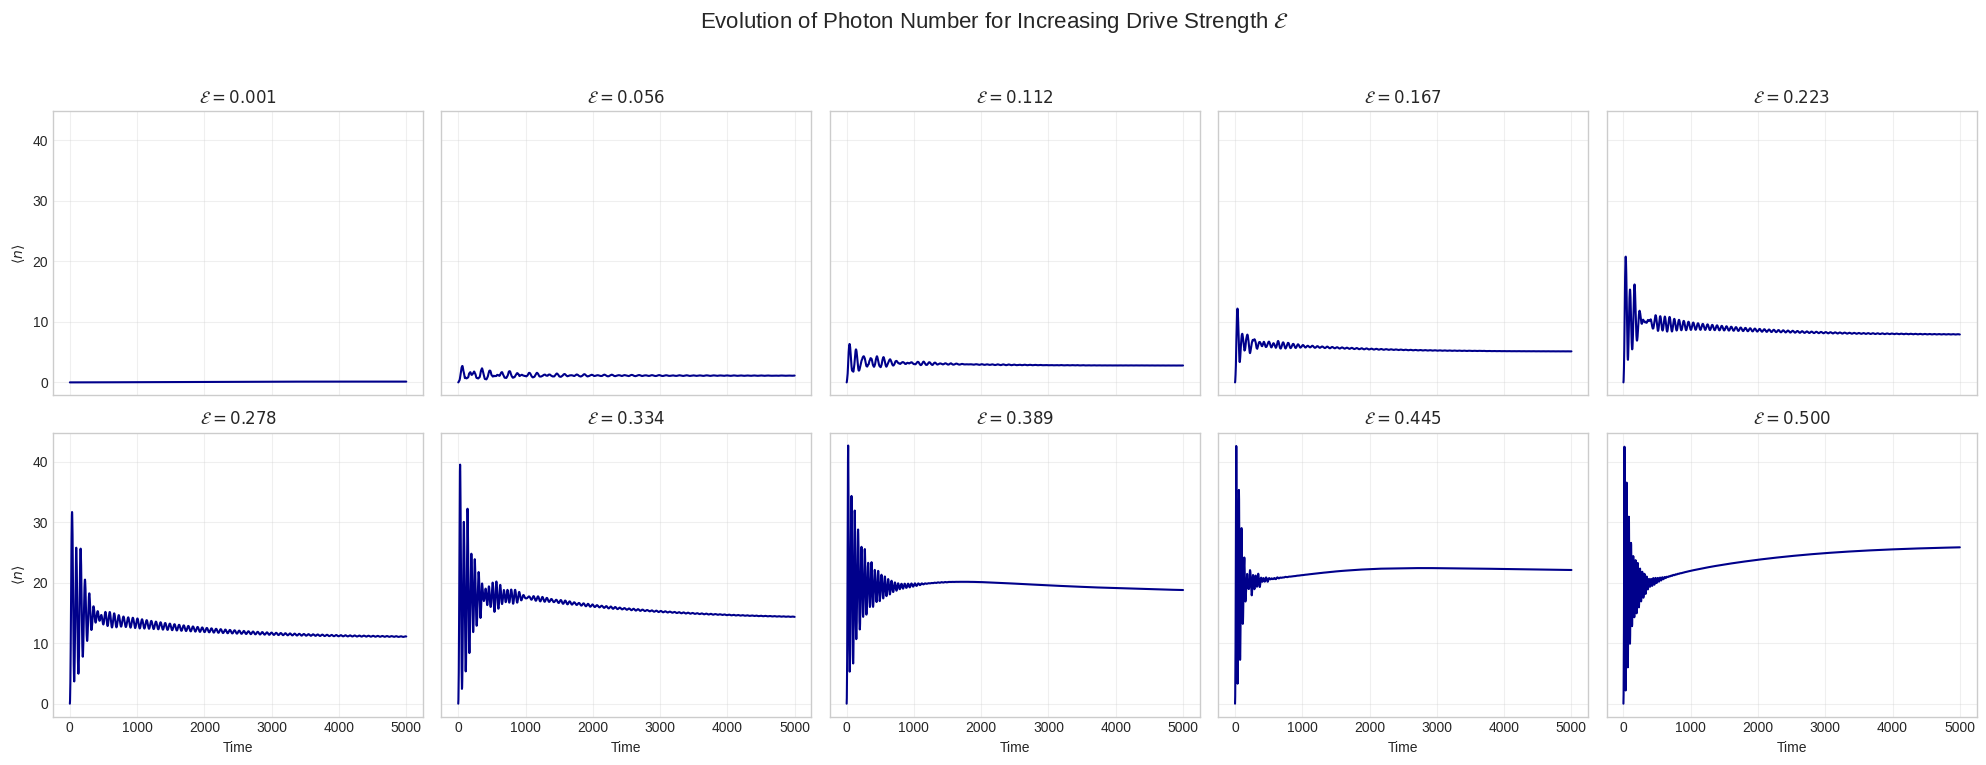
\includegraphics[width=0.75\linewidth]{Figure/E_epxect_strong.png}
    \caption{Time evolution of the mean photon number $\langle n \rangle$ for increasing drive strength $\mathcal{E}$. The system reaches a steady-state plateau where the drive is balanced by dissipation. Note that the maximum $\langle n \rangle$ remains below 0.1, illustrating the suppression of higher Fock states.}
    \label{fig:E_expect_strong}
\end{figure}

As the intensity of the drive grows, we can see that the number of photons in the cavity reaches an equilibrium state at longer times.

\begin{figure}[H]
    \centering
    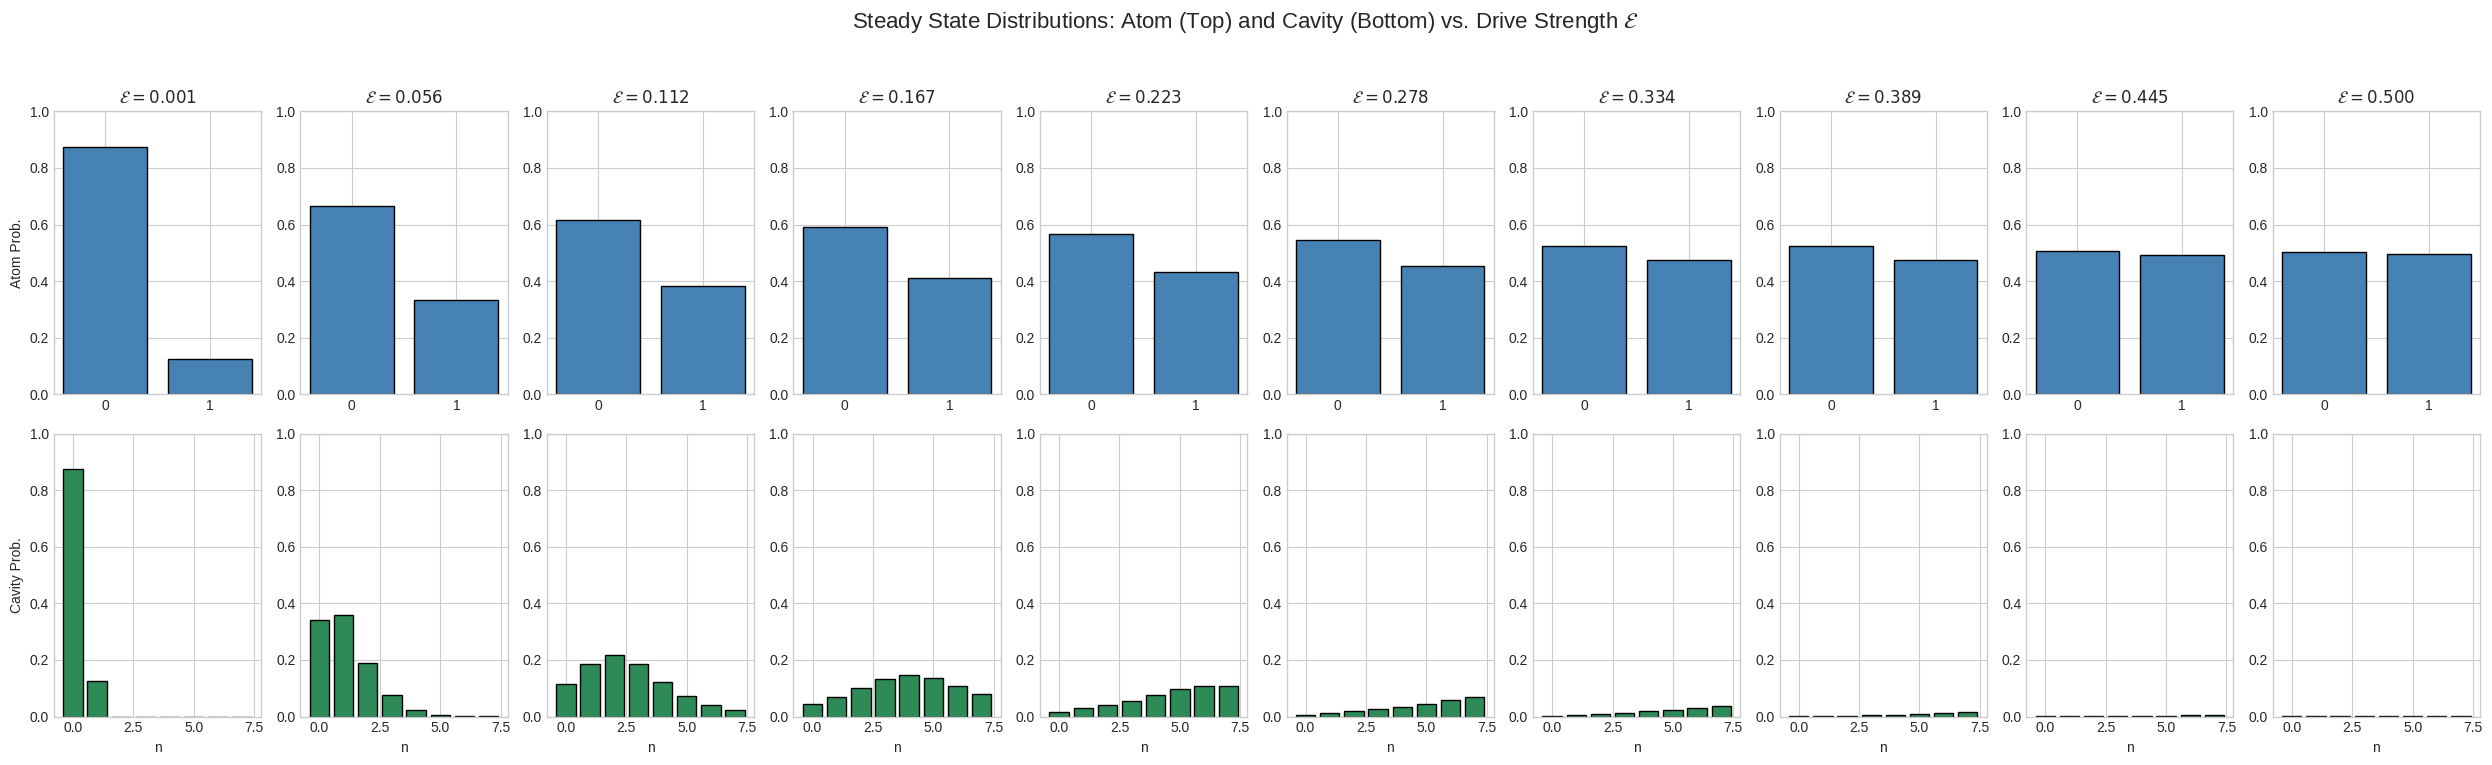
\includegraphics[width=0.75\linewidth]{Figure/E_prob_strong.png}
    \caption{Steady-state occupation probabilities for various drive strengths $\mathcal{E}$. The $n=0$ (ground) and $n=1$ (single-photon) states dominate the distribution, while the $n=2$ population remains negligible, confirming the strong blockade regime.}
    \label{fig:E_prob_strong}
\end{figure}

When looking at the distributions we gather more information since now we can see two main behaviors:
\begin{itemize}
    \item The probability of finding the atom in the excited state grows with the drive. This is expected since, driving the cavity mode necessarily populates the atomic excited state $|e\rangle$.
    \item When the drive becomes too strong compared with the dissipation rate $\kappa$, the steady-state photon number exceeds the Hilbert space cutoff. This produces an artificial flattening of the occupation distribution, which is due to numerical errors.
\end{itemize}
\subsection{Can you have occupation of two photon states? If not, why? What happens if you increase the values of the decay rates? And if you change $\tilde{g}$?}

In the strong-coupling regime with a weak drive, the occupation of two-photon states is strongly suppressed. This is the hallmark of the \textbf{photon blockade effect}. The physical reason lies in the anharmonicity of the Jaynes-Cummings energy ladder: the transition from the ground state to the first excited state $|g,0\rangle \to |1, \pm\rangle$ is resonant with the drive frequency $\omega = \omega_c \pm g$. However, due to the $\sqrt{n}$ scaling of the coupling, the transition to the two-photon state $|2, \pm\rangle$ is detuned by $(\sqrt{2}-1)g$. If this detuning is much larger than the linewidth of the states, the system cannot absorb a second photon.

\paragraph{The coupling parameter $\tilde{g}$}
Decreasing $\tilde{g}$ reduces the anharmonicity of the system. We can see that when we reach the strong coupling regime the probability of finding two photons states is 0

\begin{figure}[H]
    \centering
    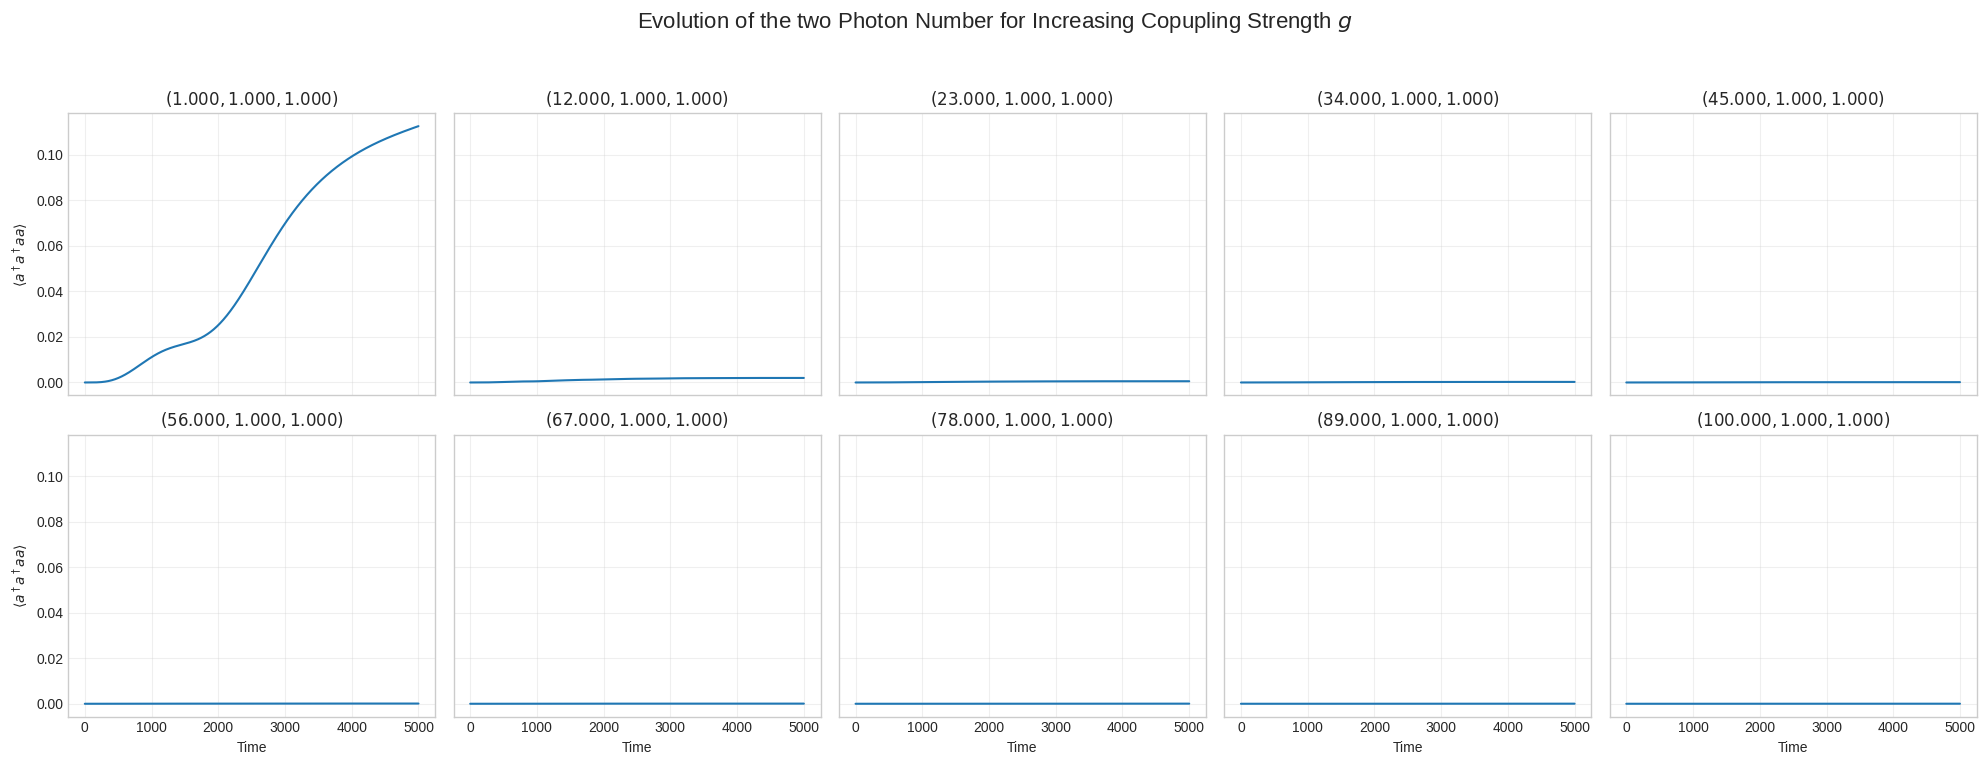
\includegraphics[width=0.75\linewidth]{Figure/g_epxect_strong.png}
    \caption{Evolution of the mean photon number $\langle n \rangle$ for different values of the coupling strength $g$. As $g$ increases, the steady-state photon number decreases, indicating a more effective blockade.}
    \label{fig:g_expect}
\end{figure}

\begin{figure}[H]
    \centering
    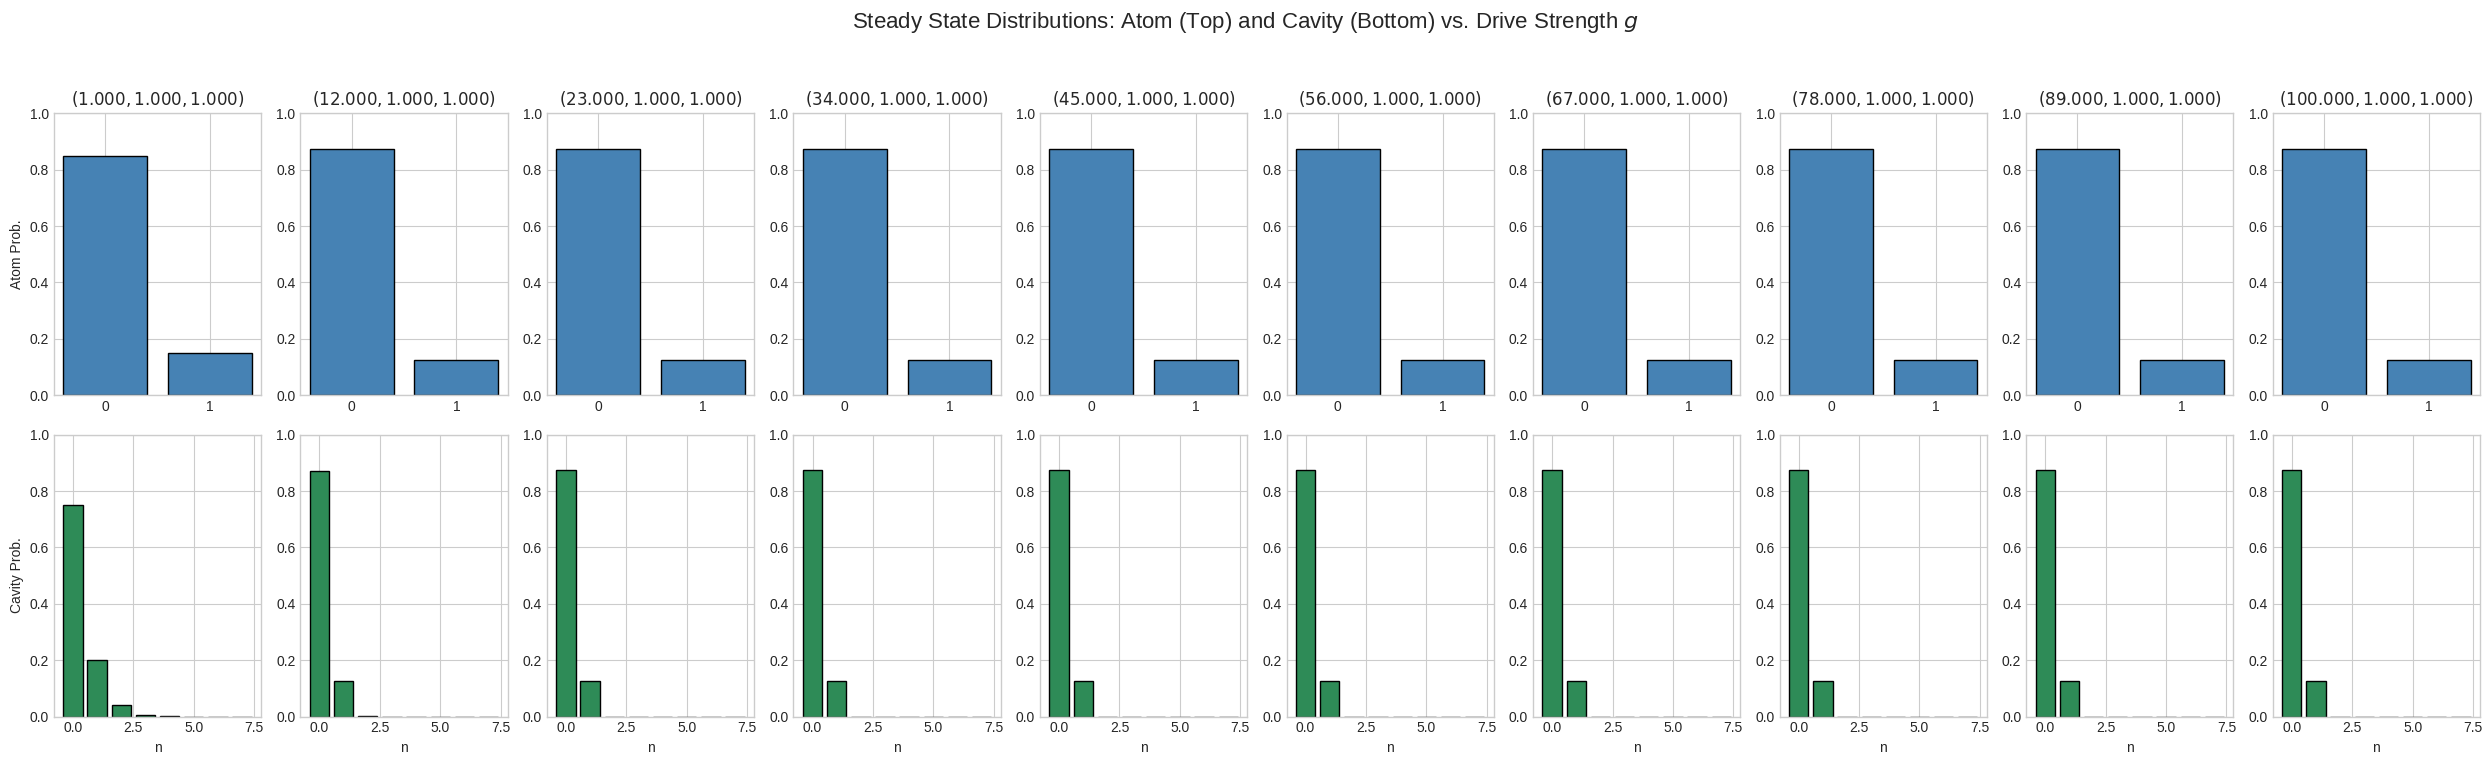
\includegraphics[width=0.75\linewidth]{Figure/g_prob_strong.png}
    \caption{Steady-state occupation probabilities for varying $g$. In the strong coupling limit (large $g$), the probability $P(n \ge 2)$ vanishes, while for small $g$ the distribution becomes more Poissonian.}
    \label{fig:g_prob}
\end{figure}

\paragraph{The coupling parameter $\kappa$}
Increasing the cavity decay rate $\kappa$ we see the opposite effect, because we are increasing the photon leaks of the bath

\begin{figure}[H]
    \centering
    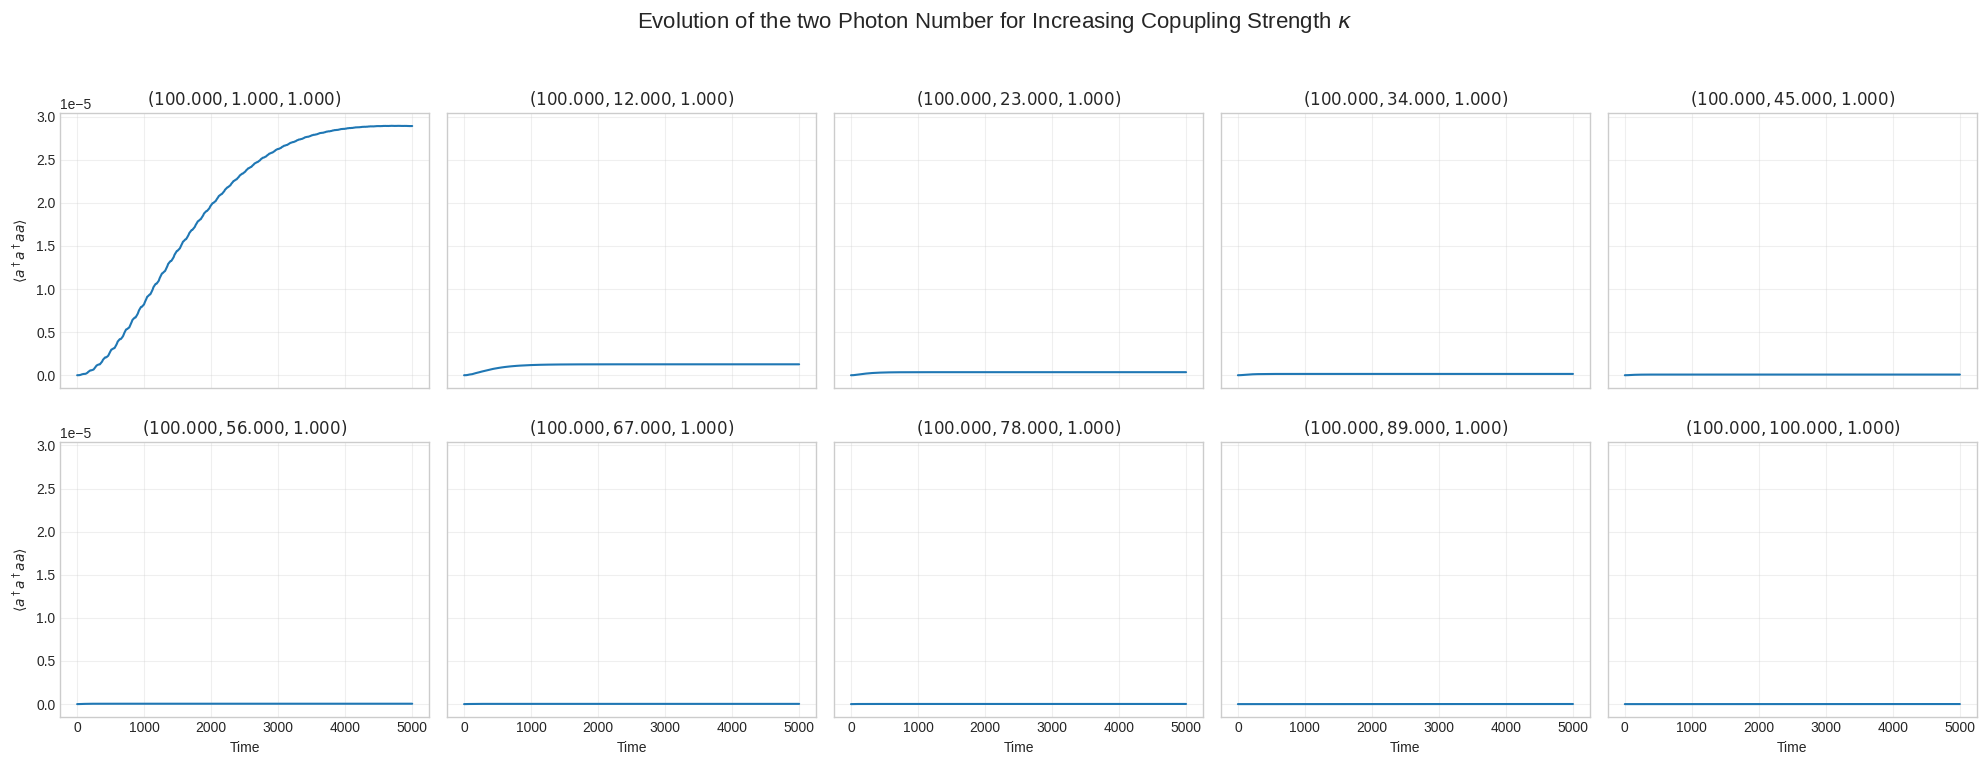
\includegraphics[width=0.75\linewidth]{Figure/k_epxect_strong.png}
    \caption{Impact of cavity dissipation $\kappa$ on the photon evolution. Higher decay rates lead to lower photon numbers but also broader resonances that degrade the blockade quality.}
    \label{fig:k_expect}
\end{figure}

\begin{figure}[H]
    \centering
    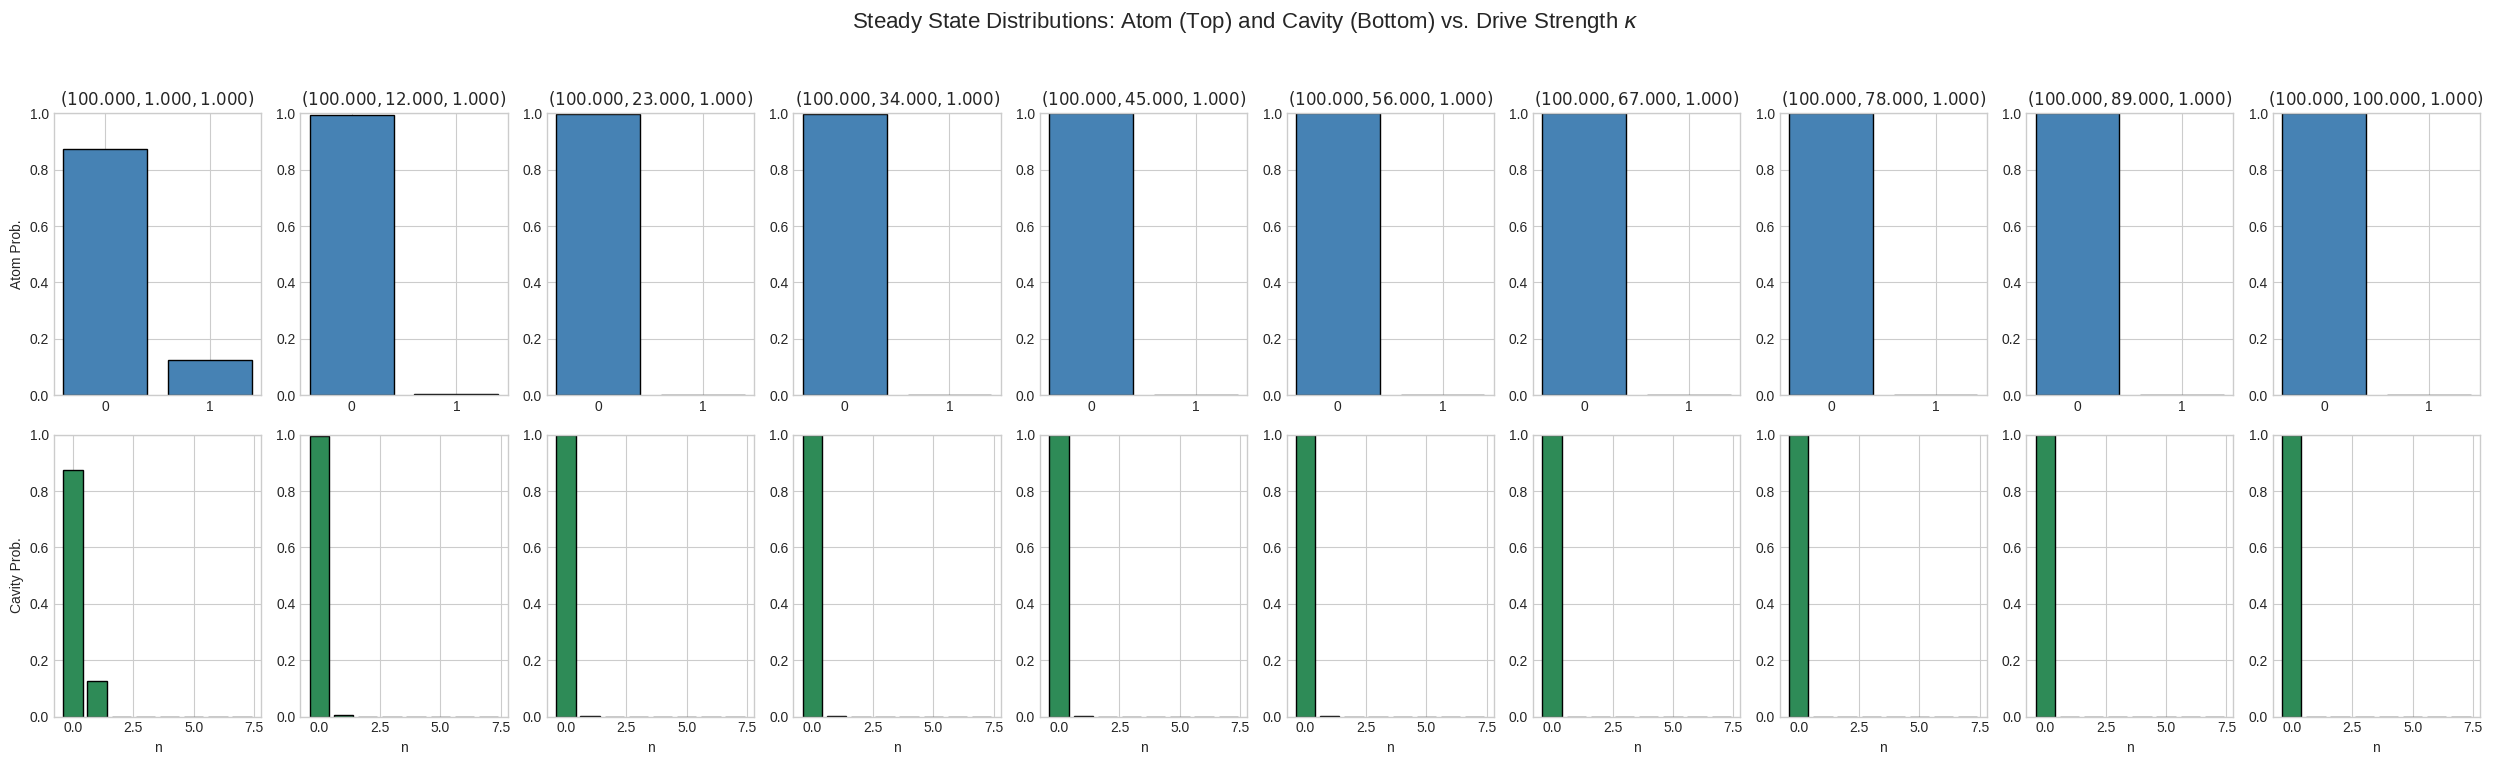
\includegraphics[width=0.75\linewidth]{Figure/k_prob_strong.png}
    \caption{Photon statistics for varying $\kappa$. Note that as $\kappa$ increases, the system transitions from a quantum blocked state toward a regime with higher statistical fluctuations.}
    \label{fig:k_prob}
\end{figure}

\paragraph{The coupling parameter $\Gamma$}
The atomic decay rate $\Gamma$ (or $\gamma$) acts similarly to $\kappa$ by introducing decoherence. A high $\Gamma$ reduces the lifetime of the atomic excitation, which effectively reduces the interaction time between the atom and the cavity field, weakening the non-linear response required for the blockade.

\begin{figure}[H]
    \centering
    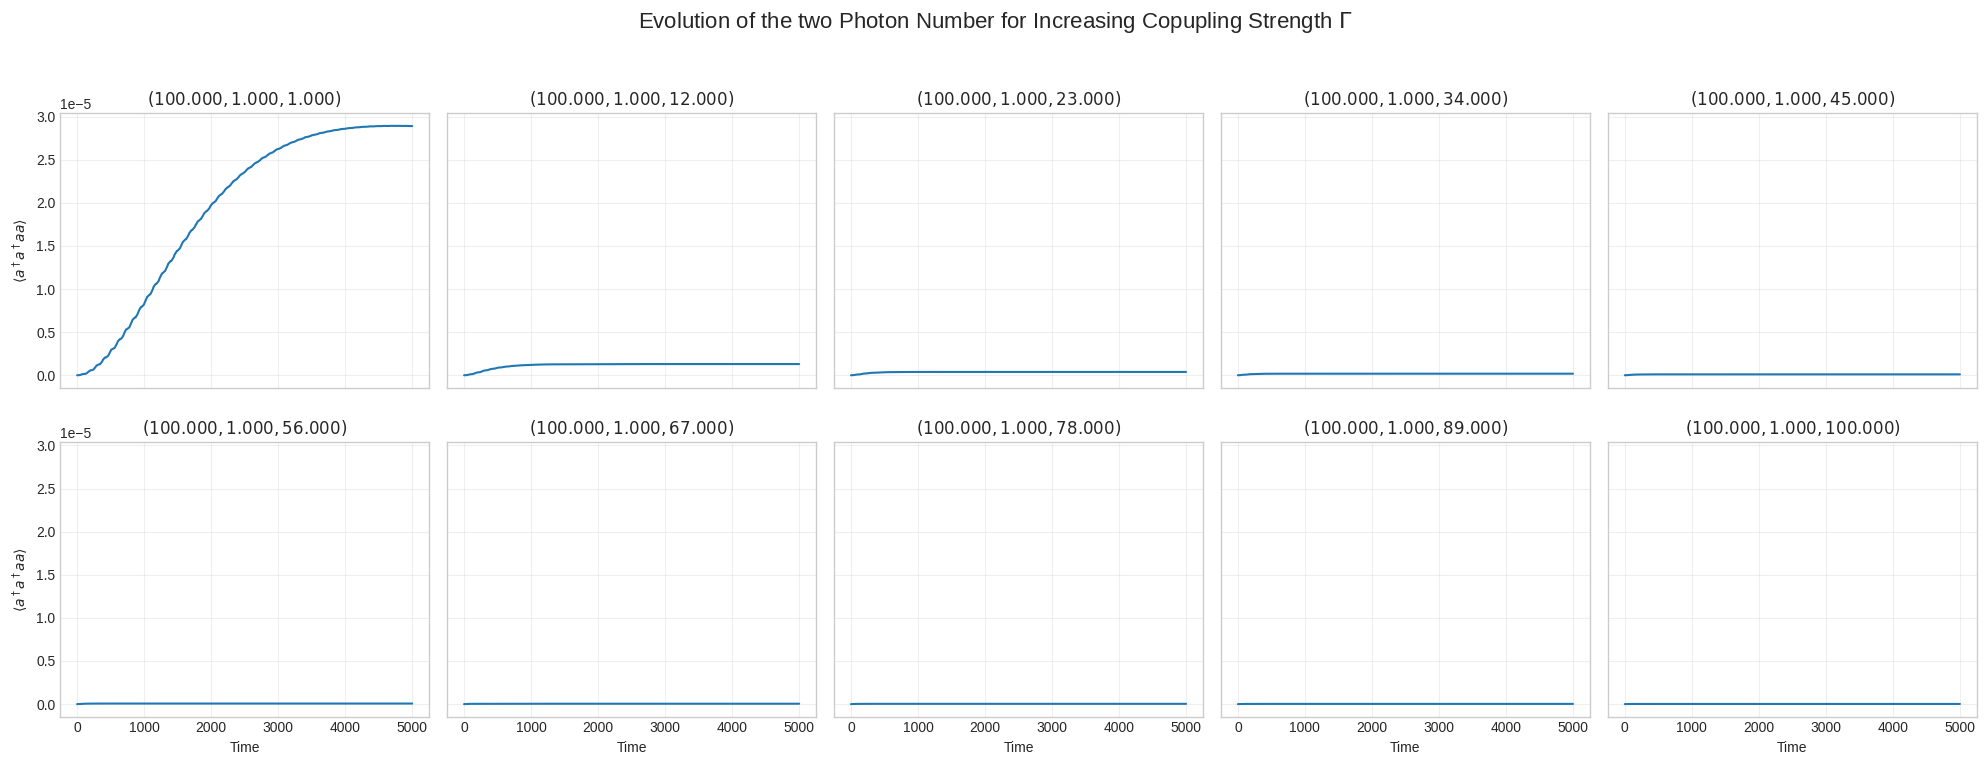
\includegraphics[width=0.75\linewidth]{Figure/G_epxect_strong.png}
    \caption{Time evolution of the expected values for varying atomic decay rates $\Gamma$. Increased atomic loss suppresses the steady-state population of the cavity mode.}
    \label{fig:G_expect}
\end{figure}

\begin{figure}[H]
    \centering
    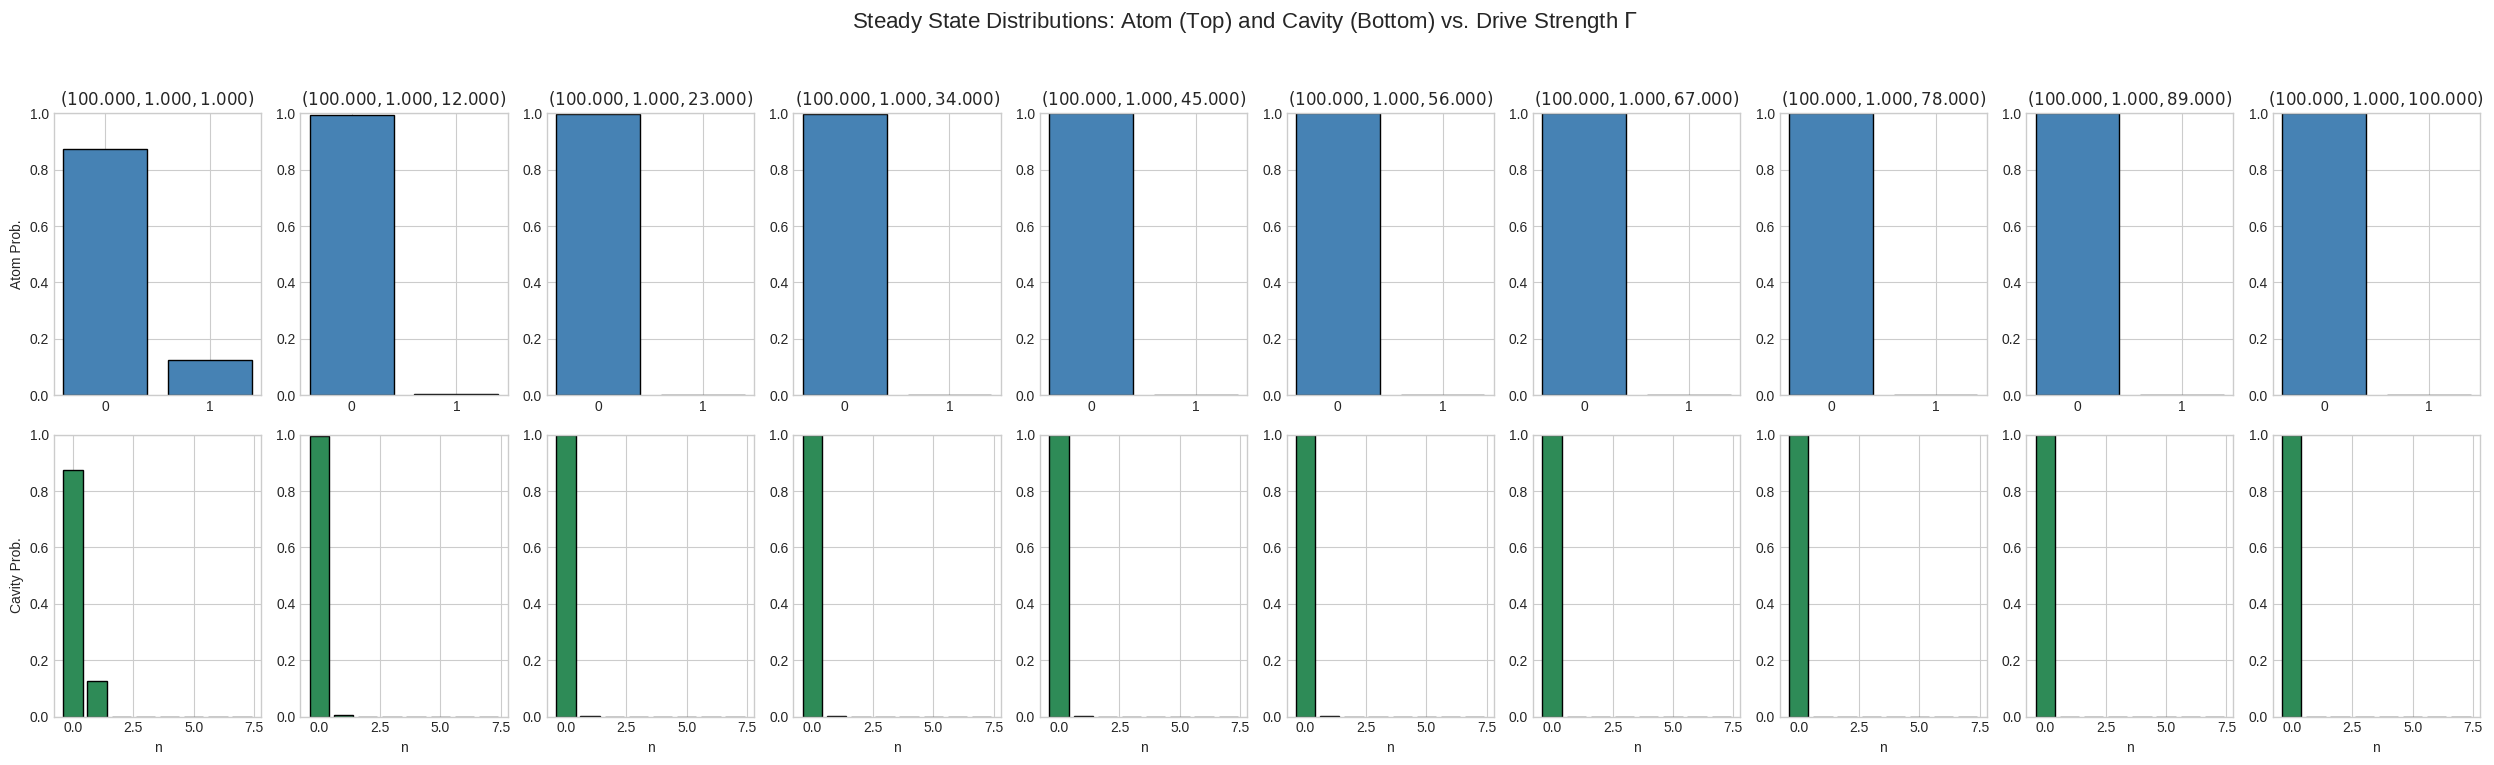
\includegraphics[width=0.75\linewidth]{Figure/G_prob_strong.png}
    \caption{Occupation probabilities as a function of $\Gamma$. The suppression of the two-photon state is most pronounced when the atomic coherence is maintained (low $\Gamma$).}
    \label{fig:G_prob}
\end{figure}

\subsection{A way to understand the suppression of two-photon states is to compute the two-photon correlation function $g^{(2)} \equiv \langle \hat{a}^\dagger \hat{a}^\dagger \hat{a} \hat{a} \rangle / \langle \hat{a}^\dagger \hat{a} \rangle^2$, which compares the probability to find two simultaneous photons with the one of having two independent photons at random. In the blockade regime, you should find $g^{(2)} < 1$.}

A convenient operational expression for the zero-delay second-order correlation is
\[
  g^{(2)}(0)
  =
  \frac{\mathrm{Tr}\left(\hat{a}^\dagger \hat{a}^\dagger \hat{a} \hat{a} \,\rho_{\mathrm{ss}}\right)}{\left[\mathrm{Tr}\left(\hat{a}^\dagger \hat{a} \,\rho_{\mathrm{ss}}\right)\right]^2}
  =
  \frac{\langle \hat{a}^\dagger \hat{a}^\dagger \hat{a} \hat{a} \rangle_{\mathrm{ss}}}{\langle \hat{a}^\dagger \hat{a} \rangle_{\mathrm{ss}}^2}
\]
where $\rho_{\mathrm{ss}}$ is the steady-state density matrix obtained by integrating the master equation until transients vanish (the cavity Hilbert space must be truncated to a sufficiently large Fock cutoff for numerical convergence).

Evaluating the steady state for the parameters used in this work gives the numerical values
\[
  \langle n \rangle = \mathrm{Tr}\left(\hat{a}^\dagger\hat{a}\\,\rho_{\mathrm{ss}}\right) = 0.1251, \qquad
  g^{(2)}(0) = 0.0018.
\]
Because $g^{(2)}(0)\ll 1$ the emitted field is strongly anti-bunched: the probability to detect two simultaneous photons is suppressed compared with independent (Poissonian) emission. This observation is the signature of the photon-blockade effect in the driven Jaynes--Cummings system: the anharmonicity of the dressed-state ladder makes the two-photon transition far less likely than the single-photon one.


\subsection{Scan the values of $\omega$ around the resonance and graphically represent your findings as in Fig. 2a of the paper by Birnbaum et al.}

To characterize the system response across the resonance, we perform a frequency scan of the driving field $\omega$ around the bare cavity resonance $\omega_c$. The resulting transmission spectrum, shown in Fig. \ref{fig:birnbaum_scan}, exhibits the classic \textbf{Vacuum Rabi Splitting}. 

The two distinct peaks are located at $\omega = \omega_c \pm g$, representing the two-component nature of the first rung of the Jaynes-Cummings ladder . In the strong-coupling regime ($\tilde{g} \gg \kappa, \Gamma$), these peaks are well-resolved and separated by a wide transparency window. This frequency-dependent response is what allows for the photon blockade: while the system is highly transparent to a single photon, the non-linearity of the interaction shifts the two-photon resonance away from these peaks, creating the suppression of the $g^{(2)}(0)$ correlation function as observed in Fig. 2a of the reference paper.

\begin{figure}[H]
    \centering
    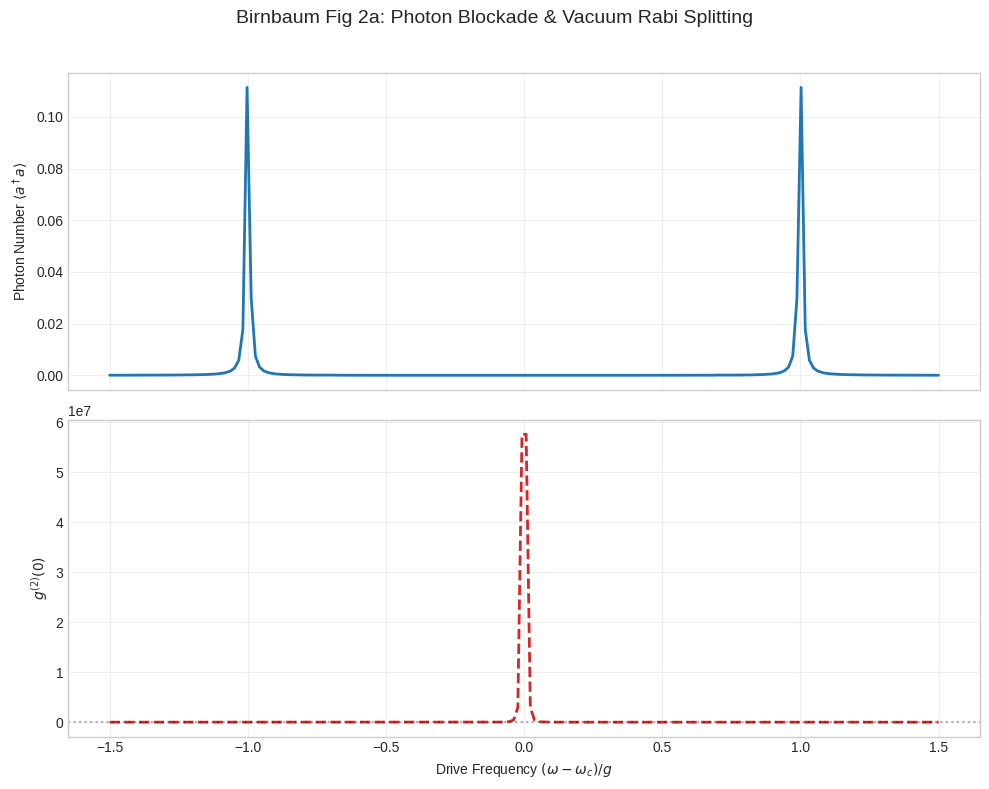
\includegraphics[width=0.75\linewidth]{Figure/B.png}
    \caption{Steady-state mean photon number $\langle \hat{a}^\dagger \hat{a} \rangle$ as a function of the drive frequency detuning $\Delta = \omega - \omega_c$. The doublet of peaks signifies the Vacuum Rabi splitting in the strong coupling regime.}
    \label{fig:birnbaum_scan}
\end{figure}


